\let\negmedspace\undefined
\let\negthickspace\undefined
\documentclass[journal]{IEEEtran}
\usepackage[a5paper, margin=10mm, onecolumn]{geometry}
%\usepackage{lmodern} % Ensure lmodern is loaded for pdflatex
\usepackage{tfrupee} % Include tfrupee package

\setlength{\headheight}{1cm} % Set the height of the header box
\setlength{\headsep}{0mm}     % Set the distance between the header box and the top of the text

\usepackage{gvv-book}
\usepackage{gvv}
\usepackage{cite}
\usepackage{amsmath,amssymb,amsfonts,amsthm}
\usepackage{algorithmic}
\usepackage{graphicx}
\usepackage{textcomp}
\usepackage{xcolor}
\usepackage{txfonts}
\usepackage{listings}
\usepackage{enumitem}
\usepackage{mathtools}
\usepackage{gensymb}
\usepackage{comment}
\usepackage[breaklinks=true]{hyperref}
\usepackage{tkz-euclide} 
\usepackage{listings}
% \usepackage{gvv}                                        
\def\inputGnumericTable{}                                 
\usepackage[latin1]{inputenc}                                
\usepackage{color}                                            
\usepackage{array}                                            
\usepackage{longtable}                                       
\usepackage{calc}  
\usepackage{amsmath,amssymb}

\usepackage{multicol}                                         
\usepackage{hhline}                                           
\usepackage{ifthen}                                           
\usepackage{lscape}
\begin{document}

\bibliographystyle{IEEEtran}

\title{
%	\logo{
NCERT - 10.4.ex.14.1

\large{EE1003}
%	}
}
\author{Homa Harshitha Vuddanti

(EE24BTECH11062)
}	

\maketitle

\bigskip

\renewcommand{\thefigure}{\theenumi}
\renewcommand{\thetable}{\theenumi}
\textbf{Question}: Find the roots of the equation : $x+\frac{1}{x}=3$, $x\neq 0$.\\
\textbf{Theoretical solution: }\\
The equation we need to solve is :
\begin{align}
    x^2-3x+1=0
\end{align}
Using the quadratic formula, the roots will be $\frac{-b\pm \sqrt{b^2-4ac}}{2a}$ for the equation $ax^2+bx+c=0$\\
Therefore, the roots are :
\begin{align}
    &\frac{3\pm \sqrt{\brak{3}^2-4\brak{1}}}{2}\\
    &\frac{3+\sqrt{5}}{2}\approx 2.61803398875,\\
    &\frac{3-\sqrt{5}}{2} \approx 0.38196601125
\end{align}
\textbf{Newton Raphson method}\\
We can use the Newton Raphson method to find the roots of the equation $x^2-3x+1=0$. The algorithm iterates as follows:
\begin{align}
x_{n+1}=x_n-\frac{f\brak{x_n}}{f^\prime\brak{x_n}}
\end{align}
We take an initial guess for the root as $x_0$ for first iteration and repeat iteration until $\abs{f\brak{x_n}}$ is very small.
\begin{align}
x_{n+1}=x_n-\brak{\frac{x_n^2-3x_n+1}{2x_n-3}}
\end{align}
I have taken $x_0=0$ and $3$ for finding the two roots. \\
\textbf{Using Companion matrix :}
For a polynomial $a_nx^n+a_{n-1}x^{n-1}+\dots +a_0$, the companion matrix is of the form -\\
\begin{align}
C=
\begin{pmatrix}
0 & 1 & 0 & \cdots & 0 \\
0 & 0 & 1 & \cdots & 0 \\
\vdots & \vdots & \vdots & \ddots & \vdots \\
0 & 0 & 0 & \cdots & 1 \\
-\frac{a_0}{a_n} & -\frac{a_1}{a_n} & -\frac{a_2}{a_n} & \cdots & -\frac{a_{n-1}}{a_n}
\end{pmatrix}
\end{align}
The eigen values of $C$ are the required roots of the polynomial.
We can apply the \textbf{QR- algorithm} to find the eigen values of the matrix.\\
We start with 
\begin{align}
    C_0=C
\end{align}
We can decompose it into a product 
\begin{align}
    C_0=Q_0R_0
\end{align}
Which are orthogonal and upper triangular matrices respectively.\\
Then 
\begin{align}
    C_1=R_0Q_0
\end{align}
We repeat this iteratively until $C_k$ becomes nearly upper triangular, and the diagonal of it will be the required roots.\\
For this question, 
\begin{align}
    C=\begin{pmatrix}
        0 & 1\\
        -1 & 3
    \end{pmatrix}
\end{align}
The eigen values obtained are plotted.
\\
\textbf{Plotting:}\\
Taking 
\begin{align}
x_0=0, 3\\
tolerance=10^{-6}\\
n=100
\end{align}
\begin{figure}[h!]
   \centering
   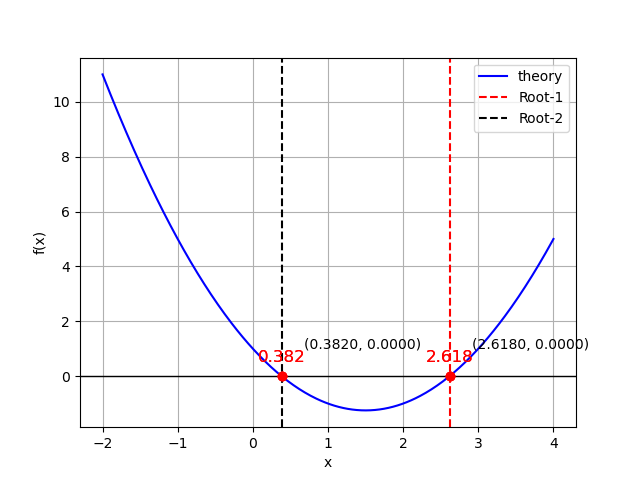
\includegraphics[width=1\columnwidth]{Figs/Figure_1.png}
   \caption{Plot}
\end{figure}
\end{document}




